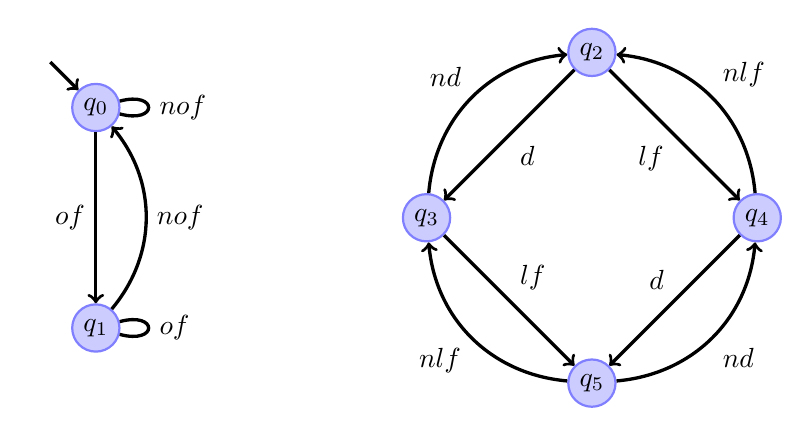
\begin{tikzpicture}[scale=0.7]
	\node 	(q0)		at	(-6,3) 	[circle, thick, draw=blue!50,fill=blue!20,inner sep=0pt,minimum size=.60cm]{$q_0$};


	\node 	(q1)		at	(-6,-1) 	[circle, thick, draw=blue!50,fill=blue!20,inner sep=0pt,minimum size=.60cm]{$q_1$}
		edge[->,very thick,bend right=40]		node[auto,swap]{$nof$}	(q0)
		edge[<-,very thick]				node[auto]{$of$}	(q0);

	\draw[loop right,very thick] (q0) to 	node[auto]{$nof$} 	(q0);
	\draw[loop right,very thick] (q1) to 	node[auto]{$of$} 	(q1);




	\node 	(q2)		at	(3,4) 	[circle, thick, draw=blue!50,fill=blue!20,inner sep=0pt,minimum size=.60cm]{$q_2$};

	\node 	(q3)		at	(0,1) 	[circle, thick, draw=blue!50,fill=blue!20,inner sep=0pt,minimum size=.60cm]{$q_3$}
		edge[->,very thick,bend left=40]		node[auto]{$nd$}	(q2)
		edge[<-,very thick]				node[auto,swap]{$d$}	(q2);


	\node 	(q4)		at	(6,1) 	[circle, thick, draw=blue!50,fill=blue!20,inner sep=0pt,minimum size=.60cm]{$q_4$}
		edge[->,very thick,bend right=40]		node[auto,swap]{$nlf$}	(q2)
		edge[<-,very thick]				node[auto]{$lf$}	(q2);

%

	\node 	(q5)		at	(3,-2) 	[circle, thick, draw=blue!50,fill=blue!20,inner sep=0pt,minimum size=.60cm]{$q_5$}
		edge[<-,very thick]				node[auto,swap]{$lf$}	(q3)
		edge[<-,very thick]				node[auto]{$d$}	(q4)
		edge[->,very thick,bend left=40]		node[auto]{$nlf$}	(q3)
		edge[->,very thick,bend right=40]		node[auto,swap]{$nd$}	(q4);


	\node 	(q)		at	(-7,4) 	[circle]{};
	\draw[->,very thick]	(q)	to node[auto,swap]{}	(q0);

\end{tikzpicture}
